% Copyright (c) 2021 Morwenn
% SPDX-License-Identifier: MIT

\documentclass{standalone}
\usepackage{bm, pgf, tikz}
\usetikzlibrary{arrows, automata, backgrounds, positioning}

\begin{document}
    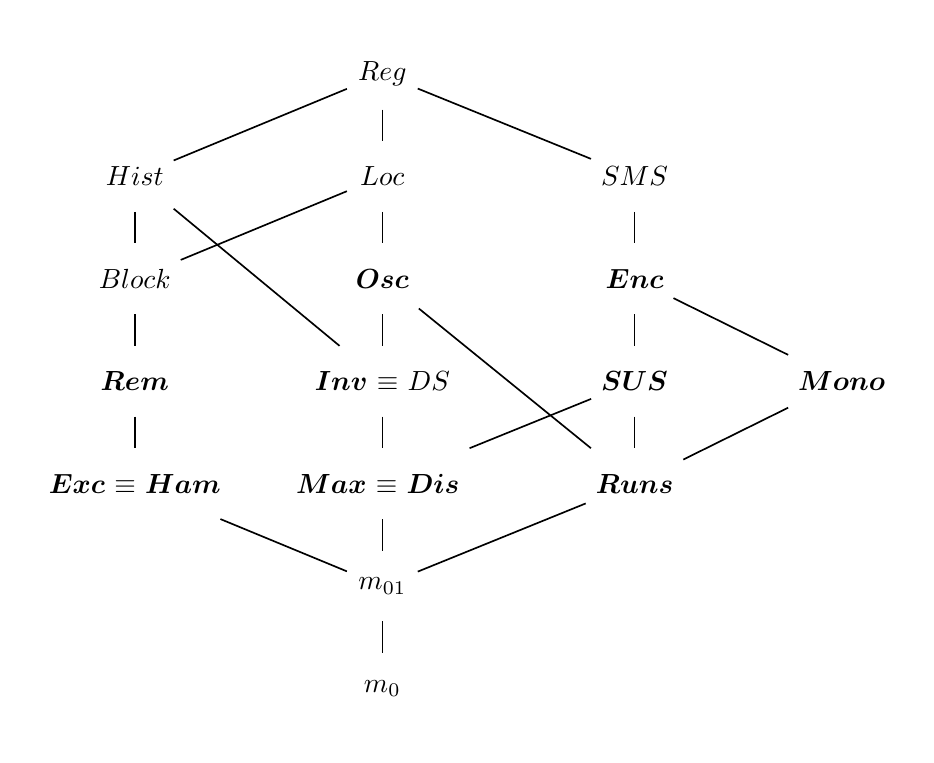
\begin{tikzpicture}[
            background rectangle/.style={fill=white},
            show background rectangle,
            auto,
            node distance = 1.3cm,
            semithick
        ]

        \tikzstyle{every state}=[
            draw=none,
            shape=rectangle,
            fill=white
        ]

        % A framework for adaptive sorting
        % by O. Pertersson and A. Moffat
        %
        % Max=Dis equivalence comes from:
        % NeatSort - A practical adaptive algorithm
        % by M. La Rocca and D. Cantone
        \node[state] (reg) {$Reg$};
        \node[state] (loc) [below of=reg] {$Loc$};
        \node[state] (hist) [left=2.2cm of loc] {$Hist$};
        \node[state] (sms) [right=2.2cm of loc] {$SMS$};
        \node[state] (block) [below of=hist] {$Block$};
        \node[state] (osc) [below of=loc] {$\bm{Osc}$};
        \node[state] (enc) [below of=sms] {$\bm{Enc}$};
        \node[state] (rem) [below of=block] {$\bm{Rem}$};
        \node[state] (inv) [below of=osc] {$\bm{Inv}~$$\equiv$$~DS$};
        \node[state] (sus) [below of=enc] {$\bm{SUS}$};
        \node[state] (exc) [below of=rem] {$\bm{Exc}~$$\equiv$$~\bm{Ham}$};
        \node[state] (max) [below of=inv] {$\bm{Max}~$$\equiv$$~\bm{Dis}~$};
        \node[state] (runs) [below of=sus] {$\bm{Runs}$};
        \node[state] (m01) [below of=max] {$m_{01}$};
        \node[state] (m0) [below of=m01] {$m_{0}$};
        \path[-] (reg) edge node {} (hist);
        \path[-] (reg) edge node {} (loc);
        \path[-] (reg) edge node {} (sms);
        \path[-] (hist) edge node {} (block);
        \path[-] (hist) edge node {} (inv);
        \path[-] (loc) edge node {} (block);
        \path[-] (loc) edge node {} (osc);
        \path[-] (sms) edge node {} (enc);
        \path[-] (block) edge node {} (rem);
        \path[-] (osc) edge node {} (inv);
        \path[-] (osc) edge node {} (runs);
        \path[-] (enc) edge node {} (sus);
        \path[-] (rem) edge node {} (exc);
        \path[-] (inv) edge node {} (max);
        \path[-] (sus) edge node {} (max);
        \path[-] (sus) edge node {} (runs);
        \path[-] (exc) edge node {} (m01);
        \path[-] (max) edge node {} (m01);
        \path[-] (runs) edge node {} (m01);
        \path[-] (m01) edge node {} (m0);

        % Sort Race
        % by H. Zhang, B. Meng and Y. Liang
        \node[state] (mono) [right=1.4cm of sus] {$\bm{Mono}$};
        \path[-] (mono) edge node {} (runs);

        % See the Original Research page of the docs
        \path[-] (enc) edge node {} (mono);

    \end{tikzpicture}
\end{document}
